%
% 2023/3/16
% JPS2023春用に作り直す.

\documentclass{standalone}
% https://latexdraw.com/plot-a-function-and-data-in-latex/

\usepackage{tikz}
\usepackage{pgfplots}

\pgfplotsset{compat = newest}
\pgfplotsset{every axis/.append style={
                    label style={font=\Large},
                    tick label style={font=\Large}
                   }}
\begin{document}
    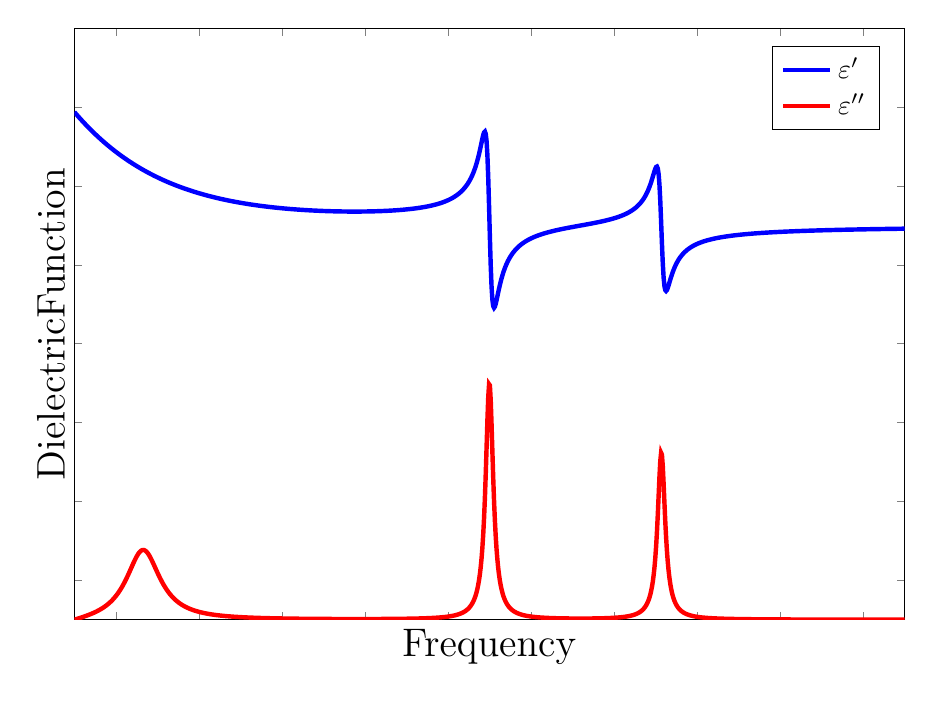
\begin{tikzpicture}
        % axis環境が2次元plot
        \begin{axis}[ %グラフ設定
%	    xmode = log,
            xmin = 0.01, xmax = 200,
            ymin = -10, ymax = 5,
            ticks=none,
	    xlabel=$\mathrm{Frequency}$,
	    ylabel=$\mathrm{Dielectric Function}$,
            % grid = both,
            minor tick num = 1,
            major grid style = {lightgray},
            minor grid style = {lightgray!25},
            width = \textwidth,
            height = 0.75\textwidth,
            legend cell align = {left},
            legend pos = north east
        ]
            %\coordinate (A) at (563,0); % additional peak @x-axis
	    %\coordinate (B) at (563,180);
            %\coordinate (C) at (598,0); % additional peak @z-axis
	    %\coordinate (D) at (598,180);
	 
	 \addplot[domain = 0.01:200,samples=1000,ultra thick,blue] {(30/(1+10*e^(0.05*x)))+1000*(10000-x*x)/((10000-x*x)*(10000-x*x)+5*x*x))+1000*(20000-x*x)/((20000-x*x)*(20000-x*x)+5*x*x))};

	 \addplot[domain = 0.01:200,samples=1000,ultra thick,red] {-10+3000*x/((300-x*x)*(300-x*x)+100*x*x)+3000*x/((10000-x*x)*(10000-x*x)+5*x*x))+3000*x/((20000-x*x)*(20000-x*x)+5*x*x))};

	 % 補助線 eps_1
	 % \addplot[domain = 0:200,samples=1000,thick,blue] {30};


%            \addplot[blue,solid, line width = 2, mark = none] table [x index=2, y index=4] {\au};
%            \addplot[red ,solid, line width = 2, mark = none] table [x index=2, y index=4] {\eu};
%	    \addplot[red, dotted, line width = 2, mark=none] coordinates {(563,0) (563,180)}; 
%	    \addplot[blue,dotted, line width = 2, mark=none] coordinates {(598,0) (598,180)};
            %\addplot[red, only marks] table [x ={x}, y = {y2}] {\table};
            %\addplot[teal, only marks, mark = x, mark size = 3pt]
            %    table [x = {x}, y = {y3}] {\table};
            \legend{$\varepsilon'$,
	            $\varepsilon''$,
	    }
	    %,
            %    Plot only with marks,
            %    Plot with other type of marks}
        \end{axis}
    \end{tikzpicture}
\end{document}

% \documentclass{standalone}

% \usepackage{tikz}
% \usepackage{pgfplots}

% \pgfplotsset{compat = newest}

% \begin{document}
%     \begin{tikzpicture}
%         \begin{axis}[
%             xmin = 0, xmax = 30,
%             ymin = -1.5, ymax = 2.0,
%             xtick distance = 2.5,
%             ytick distance = 0.5,
%             grid = both,
%             minor tick num = 1,
%             major grid style = {lightgray},
%             minor grid style = {lightgray!25},
%             width = \textwidth,
%             height = 0.5\textwidth,
%             xlabel = {$x$},
%             ylabel = {$y$},
%             legend cell align = {left},
%         ]
%             \addplot[
%                 domain = 0:30,
%                 samples = 200,
%                 smooth,
%                 thick,
%                 blue,
%             ] {exp(-x/10)*( cos(deg(x)) + sin(deg(x))/10 )};
            
%             \addplot[
%                 smooth,
%                 thin,
%                 red,
%                 dashed
%             ] file[skip first] {cosine.dat};
            
%             \legend{Plot from expression, Plot from file}
%         \end{axis}
%     \end{tikzpicture}
% \end{document}